\documentclass[tikz,border=9pt]{standalone}
\usepackage[scaled=0.95]{helvet}
\renewcommand{\familydefault}{\sfdefault}
\usepackage[europeanresistors,americanvoltages]{circuitikz}
\definecolor{TEJNavy}{HTML}{0E1733}
\definecolor{TEJGreen}{HTML}{147D55}
\definecolor{TEJBlue}{HTML}{14A8D4}
\definecolor{TEJRed}{HTML}{C62828}
\begin{document}
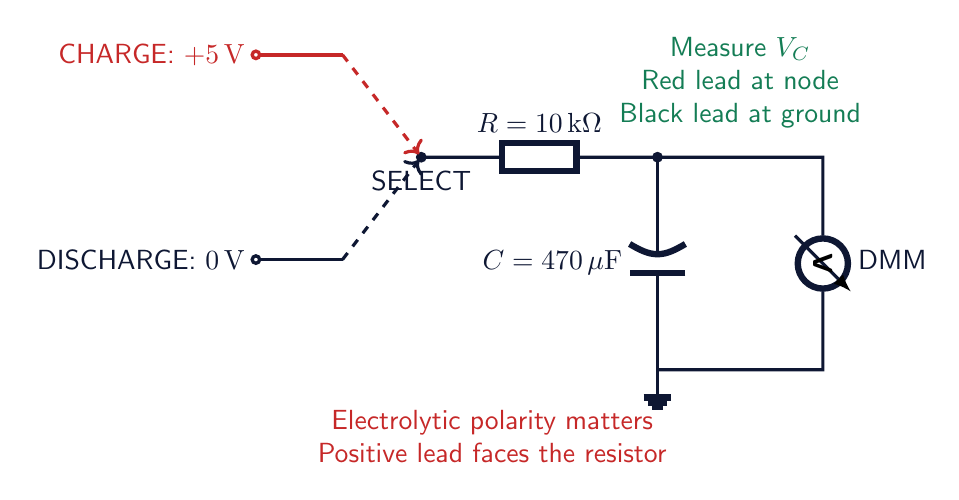
\begin{tikzpicture}[line width=1.15pt,draw=TEJNavy,text=TEJNavy,font=\sffamily]
  \ctikzset{bipoles/length=1.18cm}
  \draw[TEJRed,very thick] (0,4) node[left]{CHARGE: $+5\,\mathrm{V}$} node[ocirc]{} -- (1.1,4);
  \draw[TEJNavy,very thick] (0,1.4) node[left]{DISCHARGE: $0\,\mathrm{V}$} node[ocirc]{} -- (1.1,1.4);
  \node[circ,label=below:{SELECT}] (J) at (2.1,2.7) {};
  \draw[dashed,TEJRed,->] (1.1,4) -- (J);
  \draw[dashed,TEJNavy,->] (1.1,1.4) -- (J);
  \draw (J) to[R,l={$R=10\,\mathrm{k}\Omega$}] (5.1,2.7)
    node[circ] (Ctop) {};
  \draw (Ctop) to[polar capacitor,l_={$C=470\,\mu\mathrm{F}$}] (5.1,0)
    node[ground]{};
  \draw (Ctop) -- (7.2,2.7)
    to[voltmeter,l={DMM}] (7.2,0)
    -- (5.1,0);
  \node[TEJGreen,align=center] at (6.15,3.65)
    {Measure $V_C$\\Red lead at node\\Black lead at ground};
  \node[TEJRed,align=center] at (3.0,-0.85)
    {Electrolytic polarity matters\\Positive lead faces the resistor};
\end{tikzpicture}
\end{document}
